\documentclass[12pt, a4paper, oneside]{article}
\usepackage{amsmath, amsthm, amssymb, bm, graphicx, hyperref, mathrsfs, multirow, booktabs, makecell, tikz}
\usepackage{tikz-timing}
\usepackage{karnaugh-map}
\usepackage{circuitikz}
\usetikzlibrary{shapes,arrows,calc,arrows.meta}
\ctikzset{logic ports=ieee}
\tikzset{d-ff/.style={flipflop, flipflop def={
    t1=D, t3=C, t4={\ctikztextnot{Q}},t6=Q}}
}
\tikzset{my-ff/.style={flipflop, flipflop def={
    t1=A, t2=clk, t3=B, t4={\ctikztextnot{Q}},t6=Q}}
}
\ctikzset{
        logic ports/scale=0.7,
}
\usetikzlibrary{circuits.logic.IEC,calc}
\usetikzlibrary{automata, positioning, arrows}
\usetikztiminglibrary[rising arrows]{clockarrows}
\usepackage{xparse}
\NewDocumentCommand{\busref}{som}{\texttt{
#3
\IfValueTF{#2}{[#2]}{}
\IfBooleanTF{#1}{\#}{}
}}

\title{\textbf{Assignment\#3 CS207 Fall 2023}}
\author{Ben Chen(12212231)}
\date{\today}
\linespread{1.4}
\newcounter{problemname}
\newenvironment{problem}{\stepcounter{problemname}\par\noindent\textsc{Problem \arabic{problemname}. }}{\\\par}
\newenvironment{solution}{\par\noindent\textsc{Solution. }}{\\\par}
\newenvironment{note}{\par\noindent\textsc{Note of Problem \arabic{problemname}. }}{\\\par}

\begin{document}

\maketitle

\begin{problem}
    Analyze the sequential circuit with two JK flip-flops A and B
    with two inputs x and y and one output z.
    The input equation and output equation is given.
\end{problem}

\begin{solution}
    The state equation for the circuit is given by
    \begin{align*}
        A(t+1) &= J_A(t)A^{\prime} + K_A^{\prime}(t)A = A^{\prime}Bx + A^{\prime}B^{\prime}y^{\prime} + A(B^{\prime}xy^{\prime})^{\prime} \\
        &= A^{\prime}Bx + A^{\prime}B^{\prime}y^{\prime} + A(B+x^{\prime}+y) \\
        &= A^{\prime}Bx + A^{\prime}B^{\prime}y^{\prime} + AB + Ax^{\prime} + Ay \\
        &= \Sigma(0,2,6,7,8,9,10,12,13,14,15)
    \end{align*}
    \begin{align*}
        B(t+1) &= J_B(t)B^{\prime} + K_B^{\prime}(t)B = A^{\prime}B^{\prime}x + B(A+xy^{\prime})^{\prime} \\
        &= A^{\prime}B^{\prime}x + A^{\prime}Bx^{\prime}y \\
        &= \Sigma(2,3,4,5,7)
    \end{align*}
    and the output equation is given by
    \begin{align*}
        z(t) &= Ax^{\prime}y^{\prime} + Bx^{\prime}y^{\prime} = \Sigma(4,8,12)
    \end{align*}
    So the state table is
    \newline
    \newline
    \newline
    \begin{table}[!htbp]
        \caption{State Table}
        \centering
        \begin{tabular}{p{0.055\textwidth}<{\centering}p{0.055\textwidth}<{\centering}p{0.055\textwidth}<{\centering}p{0.055\textwidth}<{\centering}p{0.055\textwidth}<{\centering}p{0.055\textwidth}<{\centering}p{0.12\textwidth}<{\centering}p{0.055\textwidth}<{\centering}p{0.055\textwidth}<{\centering}p{0.055\textwidth}<{\centering}p{0.055\textwidth}<{\centering}}
            \toprule
            \multicolumn{2}{c}{\makecell{\textbf{Present} \\ \textbf{State}}} & \multicolumn{2}{c}{\textbf{Input}} & \multicolumn{2}{c}{\makecell{\textbf{Next} \\ \textbf{State}}} & \textbf{Output} & \multicolumn{4}{c}{\textbf{JKFF Input}} \\
            \cmidrule(lr){1-2}\cmidrule(lr){3-4}\cmidrule(lr){5-6}\cmidrule(lr){7-7}\cmidrule(lr){8-11}
            $A$ & $B$ & $x$ & $y$ & $A$ & $B$ & $z$ & $J_A$ & $K_A$ & $J_B$ & $K_B$ \\
            \midrule
            0 & 0 & 0 & 0 & 1 & 0 & 0 & 1 & 0 & 0 & 0 \\
            0 & 0 & 0 & 1 & 0 & 0 & 0 & 0 & 0 & 0 & 0 \\
            0 & 0 & 1 & 0 & 1 & 1 & 0 & 1 & 1 & 1 & 1 \\
            0 & 0 & 1 & 1 & 0 & 1 & 0 & 0 & 0 & 1 & 0 \\
            0 & 1 & 0 & 0 & 0 & 1 & 1 & 0 & 0 & 0 & 0 \\
            0 & 1 & 0 & 1 & 0 & 1 & 0 & 0 & 0 & 0 & 0 \\
            0 & 1 & 1 & 0 & 1 & 0 & 0 & 1 & 0 & 1 & 1 \\
            0 & 1 & 1 & 1 & 1 & 1 & 0 & 1 & 0 & 1 & 0 \\
            1 & 0 & 0 & 0 & 1 & 0 & 1 & 1 & 0 & 0 & 1 \\
            1 & 0 & 0 & 1 & 1 & 0 & 0 & 0 & 0 & 0 & 1 \\
            1 & 0 & 1 & 0 & 1 & 0 & 0 & 1 & 1 & 0 & 1 \\
            1 & 0 & 1 & 1 & 0 & 0 & 0 & 0 & 0 & 0 & 1 \\
            1 & 1 & 0 & 0 & 1 & 0 & 1 & 0 & 0 & 0 & 1 \\
            1 & 1 & 0 & 1 & 1 & 0 & 0 & 0 & 0 & 0 & 1 \\
            1 & 1 & 1 & 0 & 1 & 0 & 0 & 1 & 0 & 0 & 1 \\
            1 & 1 & 1 & 1 & 1 & 0 & 0 & 1 & 0 & 0 & 1 \\
            \bottomrule
        \end{tabular}
    \end{table}
    \newline
    and the state diagram and timing diagram is
    \newline
    \begin{figure}[!htbp]
        \centering
        \caption{State Diagram}
        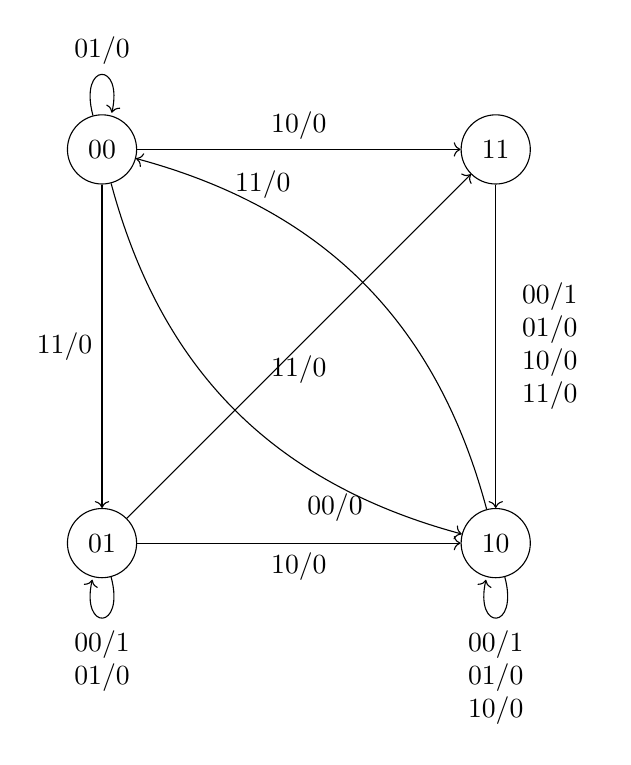
\begin{tikzpicture}[auto]
            \draw (0,0) node[state] (00) {$00$};
            \draw (0,-5) node[state] (01) {$01$};
            \draw (5,-5) node[state] (10) {$10$};
            \draw (5,0) node[state] (11) {$11$};
            \path[->]
            (00) edge [bend right] node [near end, below] {00/0} (10)
                 edge [loop above] node {01/0} (00)
                 edge node {10/0} (11)
                 edge node [left] {11/0} (01)
            (01) edge [loop below] node {\begin{tabular}{c} 00/1 \\ 01/0 \end{tabular}} (01)
                 edge node [below] {10/0} (10)
                 edge node [below] {11/0} (11)
            (10) edge [loop below] node {\begin{tabular}{c} 00/1 \\ 01/0 \\ 10/0 \end{tabular}} (10)
                 edge [bend right] node [near end, above] {11/0} (00)
            (11) edge node [right] {\begin{tabular}{c} 00/1 \\ 01/0 \\ 10/0 \\ 11/0 \end{tabular}} (10);
        \end{tikzpicture}
        \caption{Timing Diagram}
        \begin{tikztimingtable}[
            timing/dslope=0.1,
            timing/.style={x=5ex,y=2ex},
            x=5ex,
            timing/rowdist=3ex,
            timing/name/.style={font=\sffamily\scriptsize}
        ]
        \busref{CLK}         & 20{c} \\
        \busref*{$A$}      & 2L l 2H L H L 2H h \\
        \busref*{$B$}      & 3l 2H 4L H L l \\
        \busref*{$x$}       & L 4H L 2H 2L \\
        \busref*{$y$}     & L 4H L H 3L  \\
        \busref*{$z$}     & 8L l 2h l \\
        \extracode
        \begin{pgfonlayer}{background}
        \begin{scope}[semitransparent ,semithick]
        \vertlines[darkgray,dotted]{0.5,1.5 ,...,9.0,9.5}
        \end{scope}
        \end{pgfonlayer}
        \end{tikztimingtable}
    \end{figure}
\end{solution}

\begin{problem}
    Analyze the sequential circuit with two TFFs A and B.
\end{problem}

\begin{solution}
    From the diagram, we can derive the input equations
    \begin{align*}
        T_A &= A + B \\
        T_B &= A^{\prime} + B
    \end{align*}
    and there's no output equation.
    So the state equation would be
    \begin{align*}
        A(t+1) &= T_A\oplus Q_A = (A+B) \oplus A \\
        B(t+1) &= T_B\oplus Q_B = (A^{\prime}+B) \oplus B
    \end{align*}
    and the state table is
    \begin{table}[!htbp]
        \caption{State Table}
        \centering
        \begin{tabular}{p{0.1\textwidth}<{\centering}p{0.1\textwidth}<{\centering}p{0.1\textwidth}<{\centering}p{0.1\textwidth}<{\centering}}
            \toprule
            \multicolumn{2}{c}{\makecell{\textbf{Present} \\ \textbf{State}}} & \multicolumn{2}{c}{\makecell{\textbf{Next}}} \\
            \cmidrule(lr){1-2}\cmidrule(lr){3-4}
            $A$ & $B$ & $A$ & $B$ \\
            \midrule
            0 & 0 & 0 & 1 \\
            0 & 1 & 1 & 0 \\
            1 & 0 & 0 & 0 \\
            1 & 1 & 0 & 0 \\
            \bottomrule
        \end{tabular}
    \end{table}
    \newline
    the fourth state is useless. And the timing diagram and state diagram is
    \begin{figure}[!htbp]
        \centering
        \caption{Timing Diagram}
        \begin{tikztimingtable}[
            timing/dslope=0.1,
            timing/.style={x=5ex,y=2ex},
            x=5ex,
            timing/rowdist=3ex,
            timing/name/.style={font=\sffamily\scriptsize}
        ]
        \busref{CLK}         & 16{c} \\
        \busref*{$A$}      & l 3L 2H 2L l \\
        \busref*{$B$}      & l L 2H 4L l \\
        \extracode
        \begin{pgfonlayer}{background}
        \begin{scope}[semitransparent ,semithick]
        \vertlines[darkgray,dotted]{0.5,1.5 ,...,8.0}
        \end{scope}
        \end{pgfonlayer}
        \end{tikztimingtable}
    \end{figure}
    \begin{figure}[!htbp]
        \centering
        \caption{State Diagram}
        \begin{tikzpicture}[auto]
            \draw (0,0) node[state] (00) {$00$};
            \draw (0,-5) node[state] (01) {$01$};
            \draw (5,-5) node[state] (10) {$10$};
            \draw (5,0) node[state] (11) {$11$};
            \path[->]
            (00) edge node {} (01)
            (01) edge node {} (10)
            (10) edge node {} (00)
            (11) edge node {} (00);
        \end{tikzpicture} 
    \end{figure}
\end{solution}

\begin{problem}
    For the block diagram, find the state table and state diagram.
\end{problem}

\begin{solution}
    \textbf{a)} The input functions are
    \begin{align*}
        J_1 &= X \\
        K_1 &= (Q_2^{\prime}X)^{\prime} \\
        J_2 &= X \\
        K_2 &= (Q_1X)^{\prime}
    \end{align*}
    and the state equation is
    \begin{align*}
        Q_1(t+1) &= J_1Q_1^{\prime} + K_1^{\prime}Q_1 = Q_1^{\prime}X + Q_1Q_2^{\prime}X \\
        Q_2(t+1) &= J_2Q_2^{\prime} + K_2^{\prime}Q_2 = Q_2^{\prime}X + Q_1Q_2X \\
        Q_2^{\prime}(t+1) &= (X^{\prime} + Q_2)(Q_1^{\prime} + Q_2^{\prime} + X^{\prime}) \\
        &= X^{\prime} + Q_2(Q_1^{\prime} + Q_2^{\prime}) = X^{\prime} + Q_1^{\prime}Q_2
    \end{align*}
    and the output function is
    \[ F = X \oplus Q_2(t+1)^{\prime} = X\oplus (X^{\prime} + Q_1^{\prime}Q_2) \]
    so the state table is
    \begin{table}[!htbp]
        \caption{State Table}
        \centering
        \begin{tabular}{p{0.055\textwidth}<{\centering}p{0.055\textwidth}<{\centering}p{0.08\textwidth}<{\centering}p{0.12\textwidth}<{\centering}p{0.12\textwidth}<{\centering}p{0.1\textwidth}<{\centering}p{0.05\textwidth}<{\centering}p{0.05\textwidth}<{\centering}p{0.05\textwidth}<{\centering}p{0.05\textwidth}<{\centering}}
            \toprule
            \multicolumn{2}{c}{\makecell{\textbf{Present} \\ \textbf{State}}} & \textbf{Input} & \multicolumn{2}{c}{\makecell{\textbf{Next} \\ \textbf{State}}} & \textbf{Output} & \multicolumn{4}{c}{\textbf{JKFF Input}} \\
            \cmidrule(lr){1-2}\cmidrule(lr){3-3}\cmidrule(lr){4-5}\cmidrule(lr){6-6}\cmidrule(lr){7-10}
            $Q_1(t)$ & $Q_2(t)$ & $X$ & $Q_1(t+1)$ & $Q_2(t+1)$ & $F$ & $J_1$ & $K_1$ & $J_1$ & $K_1$ \\
            \midrule
            0 & 0 & 0 & 0 & 0 & 1 & 0 & 1 & 0 & 1 \\
            0 & 0 & 1 & 1 & 1 & 1 & 1 & 0 & 1 & 1 \\
            0 & 1 & 0 & 1 & 0 & 1 & 0 & 1 & 0 & 1 \\
            0 & 1 & 1 & 0 & 0 & 0 & 1 & 1 & 1 & 1 \\
            1 & 0 & 0 & 0 & 0 & 1 & 0 & 1 & 0 & 1 \\
            1 & 0 & 1 & 1 & 1 & 1 & 1 & 0 & 1 & 0 \\
            1 & 1 & 0 & 0 & 0 & 1 & 0 & 1 & 0 & 1 \\
            1 & 1 & 1 & 0 & 1 & 1 & 1 & 1 & 1 & 0 \\
            \bottomrule
        \end{tabular}
    \end{table}
    \begin{figure}[!htbp]
        \centering
        \caption{State Diagram}
        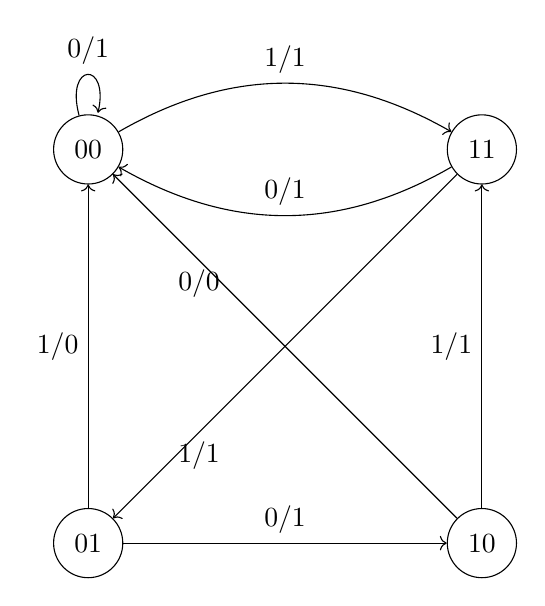
\begin{tikzpicture}[auto]
            \draw (0,0) node[state] (00) {$00$};
            \draw (0,-5) node[state] (01) {$01$};
            \draw (5,-5) node[state] (10) {$10$};
            \draw (5,0) node[state] (11) {$11$};
            \path[->]
            (00) edge [loop above] node {0/1} (00)
                 edge [bend left] node {1/1} (11)
            (01) edge node {1/0} (00)
                 edge node {0/1} (10)
            (10) edge node [near end, below] {0/0} (00)
                 edge node {1/1} (11)
            (11) edge [bend left] node [above] {0/1} (00)
                 edge node [near end, below] {1/1} (01);
        \end{tikzpicture} 
    \end{figure}
    \newline\textbf{b)} It's a Mealy Machine since the output $F$ is determined by the input $X$ and the state.
    \newline\textbf{c)} The timming diagram based on the state table is
    \begin{figure}[!htbp]
        \centering
        \caption{Timing Diagram}
        \begin{tikztimingtable}[
            timing/dslope=0.1,
            timing/.style={x=5ex,y=2ex},
            x=5ex,
            timing/rowdist=3ex,
            timing/name/.style={font=\sffamily\scriptsize}
        ]
        \busref{CLK}       & 15{c}         \\
        \busref{$X$}       & U H L 2H 2L l \\
        \busref*{$Q_1$}    & L l H L H L H L \\
        \busref*{$Q_2$}    & L l H L 2H 2L \\
        \busref*{$F$}      & U h 3H L 2H \\
        \extracode
        \begin{pgfonlayer}{background}
        \begin{scope}[semitransparent ,semithick]
        \vertlines[darkgray,dotted]{0.5,1.5 ,...,7.0}
        \end{scope}
        \end{pgfonlayer}
        \end{tikztimingtable}
    \end{figure}
\end{solution}

\begin{problem}
    Obtain the simplified input equations for a sequential circuit with TFF and the state diagram is given.
\end{problem}

\begin{solution}
    From the state diagram, we can derive the state table
    \begin{table}[!htbp]
        \caption{State Table}
        \centering
        \begin{tabular}{p{0.15\textwidth}<{\centering}p{0.15\textwidth}<{\centering}p{0.15\textwidth}<{\centering}p{0.15\textwidth}<{\centering}p{0.15\textwidth}<{\centering}}
            \toprule
            \multicolumn{2}{c}{\makecell{\textbf{Present} \\ \textbf{State}}} & \textbf{Input} & \multicolumn{2}{c}{\makecell{\textbf{Next} \\ \textbf{State}}}\\
            \cmidrule(lr){1-2}\cmidrule(lr){3-3}\cmidrule(lr){4-5}
            $Q_1(t)$ & $Q_2(t)$ & $X$ & $Q_1(t+1)$ & $Q_2(t+1)$ \\
            \midrule
            0 & 0 & 0 & 0 & 1 \\
            0 & 0 & 1 & 0 & 0 \\
            0 & 1 & 0 & 1 & 1 \\
            0 & 1 & 1 & 1 & 0 \\
            1 & 0 & 0 & 1 & 1 \\
            1 & 0 & 1 & 1 & 0 \\
            1 & 1 & 0 & 0 & 0 \\
            1 & 1 & 1 & 1 & 1 \\
            \bottomrule
        \end{tabular}
    \end{table}
    so the state equations are
    \begin{align*}
        Q_1(t+1) &= T_1 \oplus Q_1(t) = \Sigma(2,3,4,5,7) \\
        Q_2(t+1) &= T_2 \oplus Q_2(t) = \Sigma(0,2,4,7)
    \end{align*}
    and the K-Maps for each TFF are
    \begin{table}[!htbp]
        \centering
        \begin{karnaugh-map}(label=corner)[4][2][1][$X$][$Q_2$][$Q_1$]
            \minterms{2,3,4,5,7}
            \autoterms[0]
            \implicant{3}{2}
            \implicant{3}{7}
            \implicant{4}{5}
          \end{karnaugh-map}
          \begin{karnaugh-map}(label=corner)[4][2][1][$X$][$Q_2$][$Q_1$]
            \minterms{0,2,4,7}
            \autoterms[0]
            \implicantedge{0}{0}{2}{2}
            \implicant{0}{4}
            \implicant{7}{7}
        \end{karnaugh-map}
    \end{table}
    \newline So the simplified state equations are
    \begin{align*}
        Q_1(t+1) &= Q_1^{\prime}Q_2 + Q_2X + Q_1 Q_2^{\prime} \\
         &= Q_1 \oplus \left( Q_1 \oplus (Q_1^{\prime}Q_2 + Q_2X + Q_1 Q_2^{\prime}) \right) \\
         &= Q_1 \oplus (Q_1^{\prime}Q_2 + Q_1Q_2X^{\prime})
    \end{align*}
    \begin{align*}
        Q_2(t+1) &= Q_2^{\prime}X^{\prime} + Q_1^{\prime}X^{\prime} + Q_1Q_2X \\
        &= Q_2 \oplus \left(Q_2 \oplus (Q_2^{\prime}X^{\prime} + Q_1^{\prime}X^{\prime} + Q_1Q_2X)\right) \\
        &= Q_2 \oplus (Q_1Q_2X^{\prime} + Q_1^{\prime}Q_2X)
    \end{align*}
    So the input equations are
    \begin{align*}
        T_1 = Q_1^{\prime}Q_2 + Q_1Q_2X^{\prime} \\
        T_2 = Q_1Q_2X^{\prime} + Q_1^{\prime}Q_2X
    \end{align*}
\end{solution}

\begin{problem}
    Design a DFF with enable input whose function table is given.
\end{problem}

\begin{solution}
    From the characteristic table, we can derive the input equation
    \begin{figure}[!htbp]
        \centering
        \begin{karnaugh-map}(label=corner)[4][2][1][$Q$][$D$][$En$]
            \minterms{1,3,6,7}
            \autoterms[0]
            \implicant{1}{3}
            \implicant{7}{6}
          \end{karnaugh-map}
    \end{figure}
    \[ Q(t) = Q(t+1)En^{\prime} + DEn\]
    so the circuit is
    \begin{figure}[!htbp]
        \centering
        \begin{circuitikz}
            \draw (5,0) node[d-ff](FF){} (FF.up) node[above]{DFF}
            (FF.pin 1) -- ++(-0.2,0) node[or port, anchor=out](or1){}
            (FF.pin 3) -- ++(-2,0) node[left] {$Clk$}
            (or1.in 1) -- ++(-0.3,0) -- ++(0,0.3) node[and port, anchor=out](and1) {}
            (or1.in 2) -- ++(-0.3,0) -- ++(0,-0.3) node[and port, anchor=out](and2) {}
            (FF.pin 6) -- ++(0.5,0)  node[fill=black,shape=circle,scale=0.3] {} -- ++(0.7,0) node[right] {$Q$}
            (FF.pin 4) -- ++(1.2,0) node[right] {$Q^{\prime}$}
            (FF.pin 6) -- ++(0.5,0) -- ++(0,1.5) -- ++(-7,0) |- (and1.in 1)
            (and1.in 2) -- ++(-1.5,0) node[left] () {$En$}
            (and1.in 2) -- ++(-0.7,0) node[fill=black,shape=circle,scale=0.3]  {} |- (and2.in 1)
            (and2.in 1) -- ++(0.2,0) node[notcirc] () {}
            (and2.in 2) -- ++(-1.5,0) node[left] () {$D$}
            ;
        \end{circuitikz}
    \end{figure}
\end{solution}

\begin{problem}
    Design a certain filp-flop according the following description.
\end{problem}

\begin{solution}
    \textbf{a)} The characteristic table is
    \begin{table}[!htbp]
        \centering
        \begin{tabular}{p{.12\textwidth}<{\centering}p{.12\textwidth}<{\centering}p{.12\textwidth}<{\centering}p{.12\textwidth}<{\centering}p{.2\textwidth}<{\centering}}
            \toprule
            $A$ & $B$ & $Q(t+1)$ & $Q(t+1)^{\prime}$ & \\
            \midrule
            0 & 0 & 0 & 1 & clear to 0 \\
            0 & 1 & $Q(t)$ & $Q^{\prime}(t)$ & no change \\
            1 & 0 & $Q^{\prime}(t)$ & $Q(t)$ & complement \\
            1 & 1 & 1 & 0 & set to 1 \\
            \bottomrule
        \end{tabular}
    \end{table}
    \newline\textbf{b)} From the characteristic table, we can derive the K-maps first
    \begin{figure}[!htbp]
        \centering
        \begin{karnaugh-map}(label=corner)[4][2][1][$B$][$A$][$Q(t)$]
            \minterms{2,3,5,7}
            \autoterms[0]
            \implicant{3}{2}
            \implicant{5}{7}
        \end{karnaugh-map}
    \end{figure}
    \newline so the simplified equation is
    \[ Q(t+1) = AQ^{\prime}(t) + BQ(t) \]
    \textbf{c)} The excitation table is
    \begin{table}[!htbp]
        \centering
        \begin{tabular}{p{.12\textwidth}<{\centering}p{.12\textwidth}<{\centering}p{.12\textwidth}<{\centering}p{.12\textwidth}<{\centering}p{.2\textwidth}<{\centering}}
            \toprule
            $Q(t)$ & $Q(t+1)$ & $A$ & $B$ & Operation \\
            \midrule
            0 & 0 & 0 & X & no change \\
            0 & 1 & 1 & X & set to 1 \\
            1 & 0 & X & 0 & clear to 1 \\
            1 & 1 & X & 1 & no change \\
            \bottomrule
        \end{tabular}
    \end{table}
    \newline\textbf{d)} From the characteristic equation, we have
    \[ Q(t+1) = AQ^{\prime}(t) + (B^{\prime})^{\prime}Q(t) \]
    that is, we can substitude the inputs with JKFF's inputs
    \[  Q(t+1) = JQ^{\prime}(t) + K^{\prime}Q(t) \Rightarrow J = A \qquad K = B^{\prime}\]
    which is indicates the input equations of our flip-flop
    \begin{align*}
        A &= J \\
        B &= K^{\prime}
    \end{align*}
    so the block diagram is
    \begin{figure}[!htbp]
        \centering
        \begin{circuitikz}
            \draw (5,0) node[my-ff](FF){} (FF.up) node[above]{JKFF}
            (FF.pin 3) -- ++(-0.2,0) node[not port, anchor=out](not1){}
            (not1.in) -- ++(-0.6,0) node[left] {$K$}
            (FF.pin 2) -- ++(-2,0) node[left] {$Clk$}
            (FF.pin 1) -- ++(-2,0) node[left] {$J$}
            (FF.pin 6) -- ++(2,0) node[right] {$Q$}
            (FF.pin 4) -- ++(-0.2,0) node[notcirc] {} -- ++(1,0)
            ;
        \end{circuitikz}
    \end{figure}
\end{solution}

\begin{problem}
    For the following state table, simplify the state table and draw the state diagram. Then design the sequential circuit using JKFF.
\end{problem}

\begin{solution}
    To simplify the state, we first notice that the state of \textit{h} is the same as state \textit{d}, so we can remove
    the state \textit{h} and rewrite the transition to \textit{h} into \textit{d}. Then we assign codes to the states and obtain the state table
    \begin{table}[!htbp]
        \caption{State Table}
        \centering
    \begin{tabular}{p{.16\textwidth}<{\centering}p{.16\textwidth}<{\centering}p{.16\textwidth}<{\centering}p{.16\textwidth}<{\centering}p{.16\textwidth}<{\centering}}
        \toprule
        \makecell{\textbf{Present} \\ \textbf{State}} & \multicolumn{2}{c}{\makecell{\textbf{Next} \\ \textbf{State}}} & \multicolumn{2}{c}{\textbf{Output}} \\
        \cmidrule(lr){1-1}\cmidrule(lr){2-3}\cmidrule(lr){4-5}
        $ABC$ & $x=0$ & $x=1$ & $x=0$ & $x=1$\\
        \midrule
        000 & 101 & 001 & 0 & 0 \\
        001 & 011 & 010 & 0 & 0 \\
        010 & 101 & 100 & 0 & 0 \\
        011 & 110 & 000 & 1 & 0 \\
        100 & 011 & 010 & 0 & 0 \\
        101 & 101 & 010 & 1 & 1 \\
        110 & 110 & 011 & 0 & 1 \\
        111 & X & X & X & X \\
        \bottomrule
    \end{tabular}
    \end{table}
    \newline and the coresponding state diagram is
    \newline \newline
    \begin{figure}[!htbp]
        \centering
        \caption{State Diagram}
        \begin{tikzpicture}[auto]
            \draw (0,0) node[state] (000) {$000$};
            \draw (0,-3) node[state] (001) {$001$};
            \draw (0,-6) node[state] (010) {$010$};
            \draw (3,-3) node[state] (011) {$011$};
            \draw (0,-9) node[state] (100) {$100$};
            \draw (-3,-3) node[state] (101) {$101$};
            \draw (6,-3) node[state] (110) {$110$};
            \path[->]
            (000) edge node {1/0} (001)
                  edge node[above] {0/0} (101)
            (001) edge node {1/0} (010)
                  edge node {0/0} (011)
            (010) edge node {1/0} (100)
                  edge node {0/0} (101)
            (011) edge node[above] {1/0} (000)
                  edge node {0/1} (110)
            (100) edge[bend left] node {1/0} (010)
                  edge node[right] {0/0} (011)
            (101) edge[loop left] node[left] {0/1} (101)
                  edge node[above] {1/1} (001) 
            (110) edge[loop right] node[right] {0/0} (110)
                  edge[bend left] node[below] {1/1} (011);
            ;
        \end{tikzpicture} 
    \end{figure}
    \newline Next we obtain the state equations and output equation using the state table and K-map
    \begin{figure}[!htbp]
        \centering
        \begin{karnaugh-map}(label=corner)[4][4][1][$x$][$C$][$B$][$A$]
            \minterms{0,4,5,6}
            \terms{8,9,10,11,12,13,14,15}{X}
            \implicant{0}{8}
            \implicant{4}{13}
            \implicant{6}{14}
            \autoterms[0]
        \end{karnaugh-map}
        \begin{karnaugh-map}(label=corner)[4][4][1][$x$][$C$][$B$][$A$]
            \minterms{8,9,11,13}
            \terms{0,1,2,3,4,5,6,7,15,14}{X}
            \autoterms[0]
            \implicant{13}{11}
            \implicant{8}{9}
        \end{karnaugh-map}
    \end{figure}
    \begin{figure}[!htbp]
        \centering
        \begin{karnaugh-map}(label=corner)[4][4][1][$x$][$C$][$B$][$A$]
            \minterms{2,3,8,9,11}
            \terms{4,5,6,7,12,13,15,14}{X}
            \autoterms[0]
            \implicant{3}{6}
            \implicant{12}{9}
            \implicant{13}{11}
        \end{karnaugh-map}
        \begin{karnaugh-map}(label=corner)[4][4][1][$x$][$C$][$B$][$A$]
            \minterms{4,5,7}
            \terms{0,1,2,3,8,9,10,11,15,14}{X}
            \autoterms[0]
            \implicant{3}{11}
            \implicant{0}{5}
        \end{karnaugh-map}
        \begin{karnaugh-map}(label=corner)[4][4][1][$x$][$C$][$B$][$A$]
            \minterms{0,1,4,8,13}
            \terms{2,3,6,7,10,11,15,14}{X}
            \autoterms[0]
            \implicant{0}{2}
            \implicant{0}{4}
            \implicant{13}{15}
            \implicantedge{8}{8}{10}{10}
        \end{karnaugh-map}
        \begin{karnaugh-map}(label=corner)[4][4][1][$x$][$C$][$B$][$A$]
            \minterms{3,6,7,11}
            \terms{0,1,4,5,8,9,12,13,15,14}{X}
            \autoterms[0]
            \implicant{3}{11}
            \implicant{7}{14}
        \end{karnaugh-map}
    \end{figure}
    \begin{figure}[!htbp]
        \centering
        \caption{Output K-Map}
        \begin{karnaugh-map}(label=corner)[4][4][1][$x$][$C$][$B$][$A$]
            \minterms{6,10,11,13}
            \terms{14,15}{X}
            \autoterms[0]
            \implicant{13}{15}
            \implicant{6}{14}
            \implicant{15}{10}
        \end{karnaugh-map}
    \end{figure}
    \newline \newline
    \begin{table}[!htbp]
        \centering
        \caption{State Table}
        \begin{tabular}{p{.045\textwidth}<{\centering}p{.045\textwidth}<{\centering}p{.045\textwidth}<{\centering}
            p{.08\textwidth}<{\centering}p{.045\textwidth}<{\centering}p{.045\textwidth}<{\centering}p{.045\textwidth}<{\centering}
            p{.05\textwidth}<{\centering}p{.05\textwidth}<{\centering}p{.05\textwidth}<{\centering}
            p{.05\textwidth}<{\centering}p{.05\textwidth}<{\centering}p{.05\textwidth}<{\centering}}
            \toprule
            \multicolumn{3}{c}{\makecell{\textbf{Present} \\ \textbf{State}}} & \textbf{Input} & \multicolumn{3}{c}{\makecell{\textbf{Next} \\ \textbf{State}}} & \multicolumn{6}{c}{\textbf{JKFF Input}} \\
            \cmidrule(lr){1-3}\cmidrule(lr){4-4}\cmidrule(lr){5-7}\cmidrule(lr){8-13}
            $A$ & $B$ & $C$ & $x$ & $A$ & $B$ & $C$ & $J_A$ & $K_A$ & $J_B$ & $K_B$ & $J_C$ & $K_C$\\
            \midrule
            0 & 0 & 0 & 0 & 1 & 0 & 1 & 1 & X & 0 & X & 1 & X \\
            0 & 0 & 0 & 1 & 0 & 0 & 1 & 0 & X & 0 & X & 1 & X \\
            0 & 0 & 1 & 0 & 0 & 1 & 1 & 0 & X & 1 & X & X & 0 \\
            0 & 0 & 1 & 1 & 0 & 1 & 0 & 0 & X & 1 & X & X & 1 \\
            0 & 1 & 0 & 0 & 1 & 0 & 1 & 1 & X & X & 1 & 1 & X \\
            0 & 1 & 0 & 1 & 1 & 0 & 0 & 1 & X & X & 1 & 0 & X \\
            0 & 1 & 1 & 0 & 1 & 1 & 0 & 1 & X & X & 0 & X & 1 \\
            0 & 1 & 1 & 1 & 0 & 0 & 0 & 0 & X & X & 1 & X & 1 \\
            1 & 0 & 0 & 0 & 0 & 1 & 1 & X & 1 & 1 & X & 1 & X \\
            1 & 0 & 0 & 1 & 0 & 1 & 0 & X & 1 & 1 & X & 0 & X \\
            1 & 0 & 1 & 0 & 1 & 0 & 1 & X & 0 & 0 & X & X & 0 \\
            1 & 0 & 1 & 1 & 0 & 1 & 0 & X & 1 & 1 & X & X & 1 \\
            1 & 1 & 0 & 0 & 1 & 1 & 0 & X & 0 & X & 0 & 0 & X \\
            1 & 1 & 0 & 1 & 0 & 1 & 1 & X & 1 & X & 0 & 1 & X \\
            1 & 1 & 1 & X & X & X & X & X & X & X & X & X & X \\
            \bottomrule
        \end{tabular}
    \end{table}
    \newline so the input equations are
    \begin{align*}
        J_A &= C^{\prime}x^{\prime} + BC^{\prime} + BCx^{\prime} \\
        K_A &= Ax + AB^{\prime}C^{\prime} \\
        J_B &= A^{\prime}C + AC^{\prime} + Ax \\
        K_B &= A^{\prime}C^{\prime} Cx
    \end{align*}
    \begin{align*}
        J_C &= A^{\prime}B^{\prime} + A^{\prime}C^{\prime}x^{\prime} + ABx + AB^{\prime}x^{\prime} \\
        K_C &= Cx + BC
    \end{align*}
    and the output equation is
    \[ y = AC + ABx + BCx^{\prime}\]
    and the state equations are
    \begin{align*}
        A(t+1) &= J_A A^{\prime} + K_A^{\prime}A \\
        &= A^{\prime}(C^{\prime}x^{\prime} + BC^{\prime} + BCx^{\prime}) + A(Ax + AB^{\prime}C^{\prime})^{\prime} \\
        &= A^{\prime}C^{\prime}x^{\prime} + A^{\prime}BC^{\prime} + A^{\prime}BCx^{\prime} + ABx^{\prime} + ACx^{\prime} \\
        B(t+1) &= J_B B^{\prime} + K_B^{\prime}B \\
        &= B^{\prime}(A^{\prime}C + AC^{\prime} + Ax) + A(A^{\prime}C^{\prime}Cx)^{\prime} \\
        &= A + A^{\prime}B^{\prime}C \\
        C(t+1) &= J_C C^{\prime} + K_C^{\prime}C \\
        &= C^{\prime}(A^{\prime}B^{\prime} + A^{\prime}C^{\prime}x^{\prime} + ABx + AB^{\prime}x^{\prime}) + C(Cx + BC)^{\prime} \\
        &= A^{\prime}B^{\prime}C^{\prime} + A^{\prime}C^{\prime}x^{\prime} + ABC^{\prime}x + AB^{\prime}C^{\prime}x^{\prime} + BCx
    \end{align*}
\end{solution}

\begin{problem}
    Design a sequence detector using DFF to recognize the occurrence of bits 1101 with Moore machine in overlapping mode.
\end{problem}

\begin{solution}
    According to the description, we can draw the state diagram
    \newline\newline\newline\newline\newline\newline
    \begin{figure}[!htbp]
        \centering
        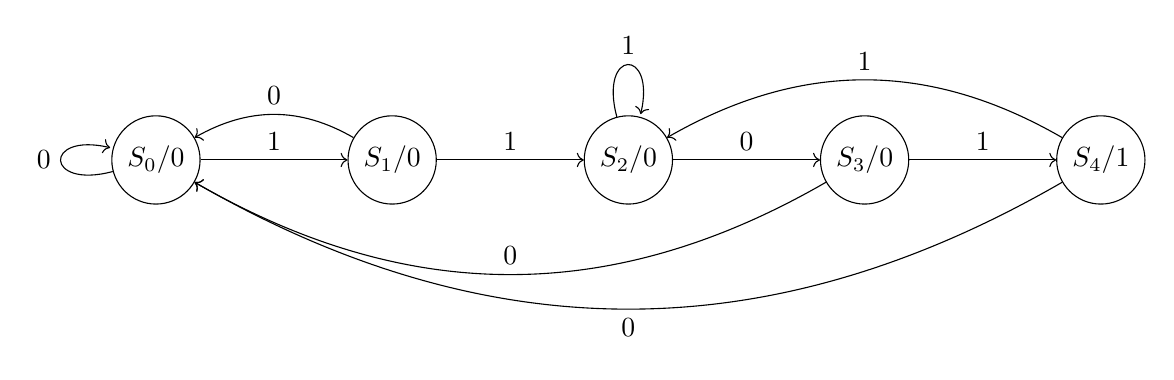
\begin{tikzpicture}[auto]
            \draw (0,0) node[state] (000) {$S_0/0$};
            \draw (3,0) node[state] (001) {$S_1/0$};
            \draw (6,0) node[state] (010) {$S_2/0$};
            \draw (9,0) node[state] (011) {$S_3/0$};
            \draw (12,0) node[state] (100) {$S_4/1$};
            \path[->]
            (000) edge node {1} (001)
                  edge[loop left] node {0} (000)
            (001) edge node {1} (010)
                  edge[bend right] node[above] {0} (000)
            (010) edge node {0} (011)
                  edge[loop above] node {1} (010)
            (011) edge node {1} (100)
                  edge[bend left] node[above] {0} (000)
            (100) edge[bend right] node[above] {1} (010)
                  edge[bend left] node {0} (000)
            ;
        \end{tikzpicture} 
    \end{figure}
    \newline and the state table is
    \begin{table}[!htbp]
        \caption{State Table}
        \centering
    \begin{tabular}{p{.25\textwidth}<{\centering}p{.2\textwidth}<{\centering}p{.2\textwidth}<{\centering}p{.2\textwidth}<{\centering}}
        \toprule
        \makecell{\textbf{Present} \\ \textbf{State}} & \multicolumn{2}{c}{\makecell{\textbf{Next} \\ \textbf{State}}} & {Output} \\
        \cmidrule(lr){1-1}\cmidrule(lr){2-3}\cmidrule(lr){4-4}
        $ABC$ & $x=0$ & $x=1$ & $y$\\
        \midrule
        ($S_0$) 000 & 000 & 001 & 0 \\
        ($S_1$) 001 & 000 & 010 & 0 \\
        ($S_2$) 010 & 011 & 010 & 0 \\
        ($S_3$) 011 & 000 & 100 & 0 \\
        ($S_4$) 100 & 000 & 010 & 1 \\
        101 & X & X & X \\
        110 & X & X & X \\
        111 & X & X & X \\
        \bottomrule
    \end{tabular}
    \end{table}
    \newline So we can obtain the input and state equations from the K-maps
    \begin{align*}
        A(t+1) &= D_A(t) = BCx\\
        B(t+1) &= D_B(t) = BC^{\prime} + Ax + B^{\prime}Cx \\
        C(t+1) &= D_C(t) = BC^{\prime}x^{\prime} + A^{\prime}B^{\prime}C^{\prime}x
    \end{align*}
    and the output equation is
    \[ y = A \]
    And the K-maps are
    \newline
    \begin{figure}[!htbp]
        \centering
        \begin{karnaugh-map}(label=corner)[4][4][1][$x$][$C$][$B$][$A$]
            \minterms{7}
            \terms{10,11,12,13,14,15}{X}
            \autoterms[0]
            \implicant{7}{15}
        \end{karnaugh-map}
        \begin{karnaugh-map}(label=corner)[4][4][1][$x$][$C$][$B$][$A$]
            \minterms{3,4,5,9}
            \terms{10,11,12,13,14,15}{X}
            \autoterms[0]
            \implicant{4}{13}
            \implicant{13}{11}
            \implicantedge{3}{3}{11}{11}
        \end{karnaugh-map}
        \begin{karnaugh-map}(label=corner)[4][4][1][$x$][$C$][$B$][$A$]
            \minterms{1,4}
            \terms{10,11,12,13,14,15}{X}
            \autoterms[0]
            \implicant{4}{12}
            \implicant{1}{1}
        \end{karnaugh-map}
        \begin{karnaugh-map}(label=corner)[4][4][1][$x$][$C$][$B$][$A$]
            \minterms{9,8}
            \terms{10,11,12,13,14,15}{X}
            \autoterms[0]
            \implicant{12}{10}
        \end{karnaugh-map}
    \end{figure}
\end{solution}

\end{document}
